%% LaTeX-Beamer template for KIT design
%% by Erik Burger, Christian Hammer
%% title picture by Klaus Krogmann
%%
%% version 2.4
%%
%% mostly compatible to KIT corporate design v2.0
%% http://intranet.kit.edu/gestaltungsrichtlinien.php
%%
%% Problems, bugs and comments to
%% burger@kit.edu

%% Class options
%%   aspect ratio options: 
%%   -- 16:9 (default)
%%   -- 4:3
%%   language options: 
%%   -- en (default)
%%   -- de
%%   position of navigation bar:
%%   -- navbarinline (default): bottom of the white canvas
%%   -- navbarinfooter : more compressed variant inside the footer
%%   -- navbarside : side bar at the left of the white canvas
%%   -- navbaroff : none
%% example: \documentclass[16:9,de,navbarinfooter]{sdqbeamer}
\documentclass[16:9,en,navbarinfooter]{sdqbeamer}

%% \documentclass{sdqbeamer} 

%% TITLE PICTURE

% if a custom picture is to be used on the title page, copy it into the 'logos'
% directory, in the line below, replace 'myimage' with the 
% filename (without extension) and uncomment the following line
% (picture proportions: 63 : 20 for standard, 169 : 40 for wide
% *.eps format if you use latex+dvips+ps2pdf, 
% *.jpg/*.png/*.pdf if you use pdflatex)

% \titleimage{myimage}

%% GROUP LOGO 

% for a custom group logo, copy your file into the 'logos'
% directory, insert the filename in the line below and uncomment it

\grouplogo{irlalr}

% (*.eps format if you use latex+dvips+ps2pdf,
% *.jpg/*.png/*.pdf if you use pdflatex)

%% GROUP NAME

% for groups other than SDQ, please insert in the line below and uncomment it
% \groupname{My group}

% the presentation starts here 

\author{Caspar Friedrich Maximilian Nagy}

%% Title (and possibly subtitle) of the thesis
\title{Solving Real-World Robot Manipulation Tasks with Deep Reinforcement Learning}
\subtitle{Box Pushing with Motion Primitives on a real Panda Robot}

% Bibliography 
\usepackage{dsfont}
\usepackage{multimedia}
%\usepackage{media9}
\usepackage{booktabs}
\usepackage{longtable}
\usepackage{array}
\usepackage{algorithm}
\usepackage{algpseudocode}
\usepackage{pgfplots}
% \pgfplotsset{compat=1.15}
 \usepgfplotslibrary{groupplots}
\usepackage{subcaption}
\usepackage{pdflscape}
\usepackage{diagbox}
\usepackage{multicol}
\DeclareUnicodeCharacter{2212}{−}
\usepgfplotslibrary{groupplots,dateplot}
\usetikzlibrary{patterns,shapes.arrows}
\pgfplotsset{compat=newest}
\usepackage[citestyle=authoryear,bibstyle=numeric,hyperref,backend=biber%,style=verbose
]{biblatex}
\addbibresource{presentation.bib}
\bibhang1em
\usepackage{listings}
\begin{document}

%title page
\KITtitleframe{}

%table of
% \begin{frame}
%     \frametitle{Video Example}
%     Here is a video:
% 
%     %\movie[width=0.6\linewidth, height=0.45\linewidth, poster, showcontrols]{Click to play}{media/test.mp4}
%     \begin{columns}
%         \column{.6\textwidth}
%     \movie[width=\linewidth, height=0.5625\linewidth, poster, showcontrols]{Click to play}{media/test.mov}
%         \column{.4\textwidth}
%     \end{columns}
% \end{frame}

\begin{frame}
	\frametitle{Agenda}
	\vspace{1cm}
	\setcounter{tocdepth}{1}
	\tableofcontents
\end{frame}

\section{Motion Primitive-Based (Re-)Planning Policy (MP3)}
\begin{frame}{Motion Primitive-Based (Re-)Planning Policy (MP3)}

	\center
	\vspace{1cm}
	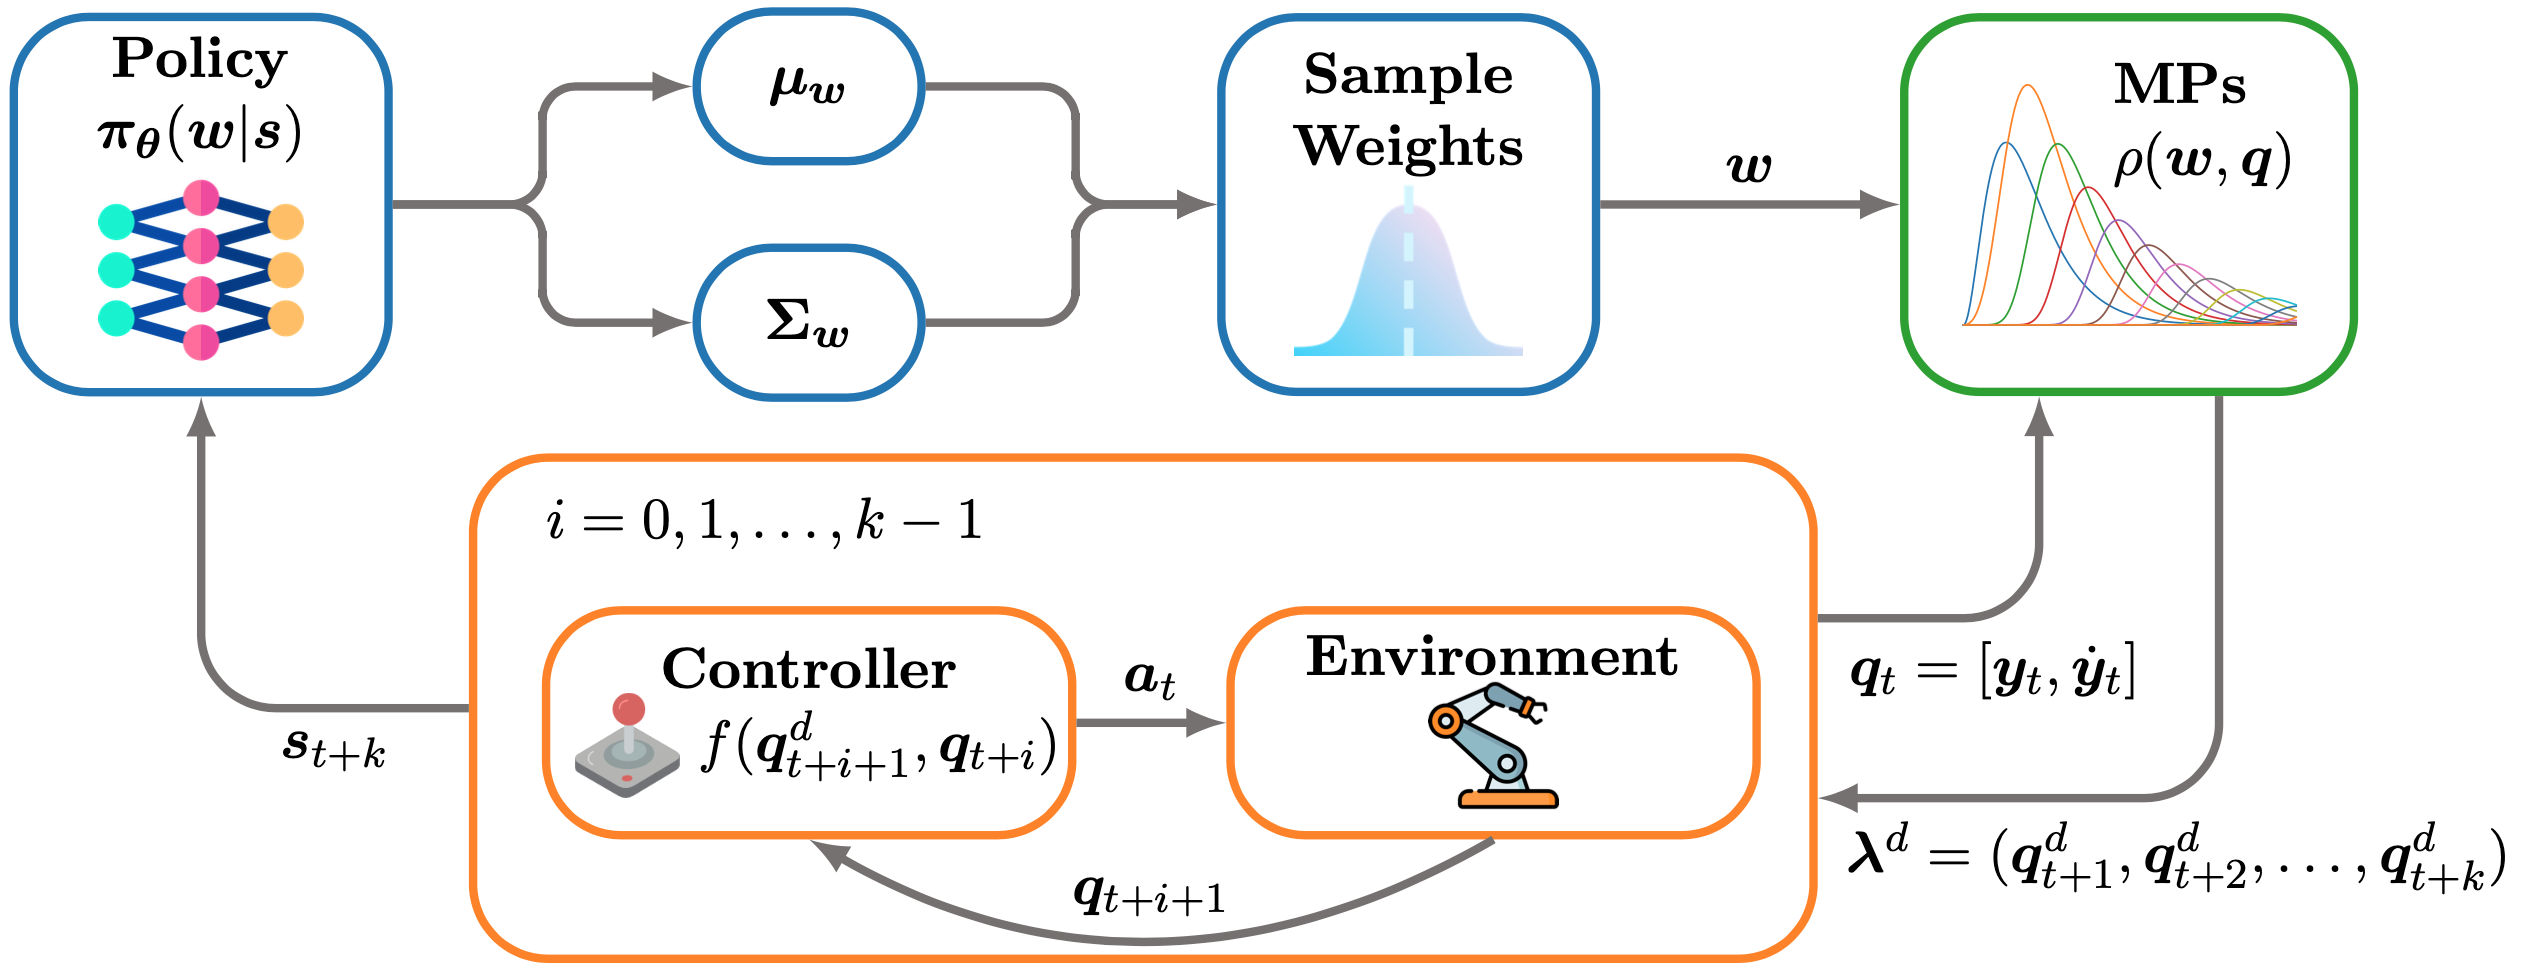
\includegraphics[width=.7\linewidth]{media/mp3.png}
	\begin{itemize}
		\item Blackbox and replanning variant
		\item Works with sparse, non-markovian rewards
		\item Generates smooth trajectories
		\item Trained on-policy using Trust Region Projection Layers (TRPL)
	\end{itemize}
\end{frame}

\subsection{MP3 in the Real World}
\begin{frame}{MP3 in the Real World}

	\center
	\vspace{1cm}
	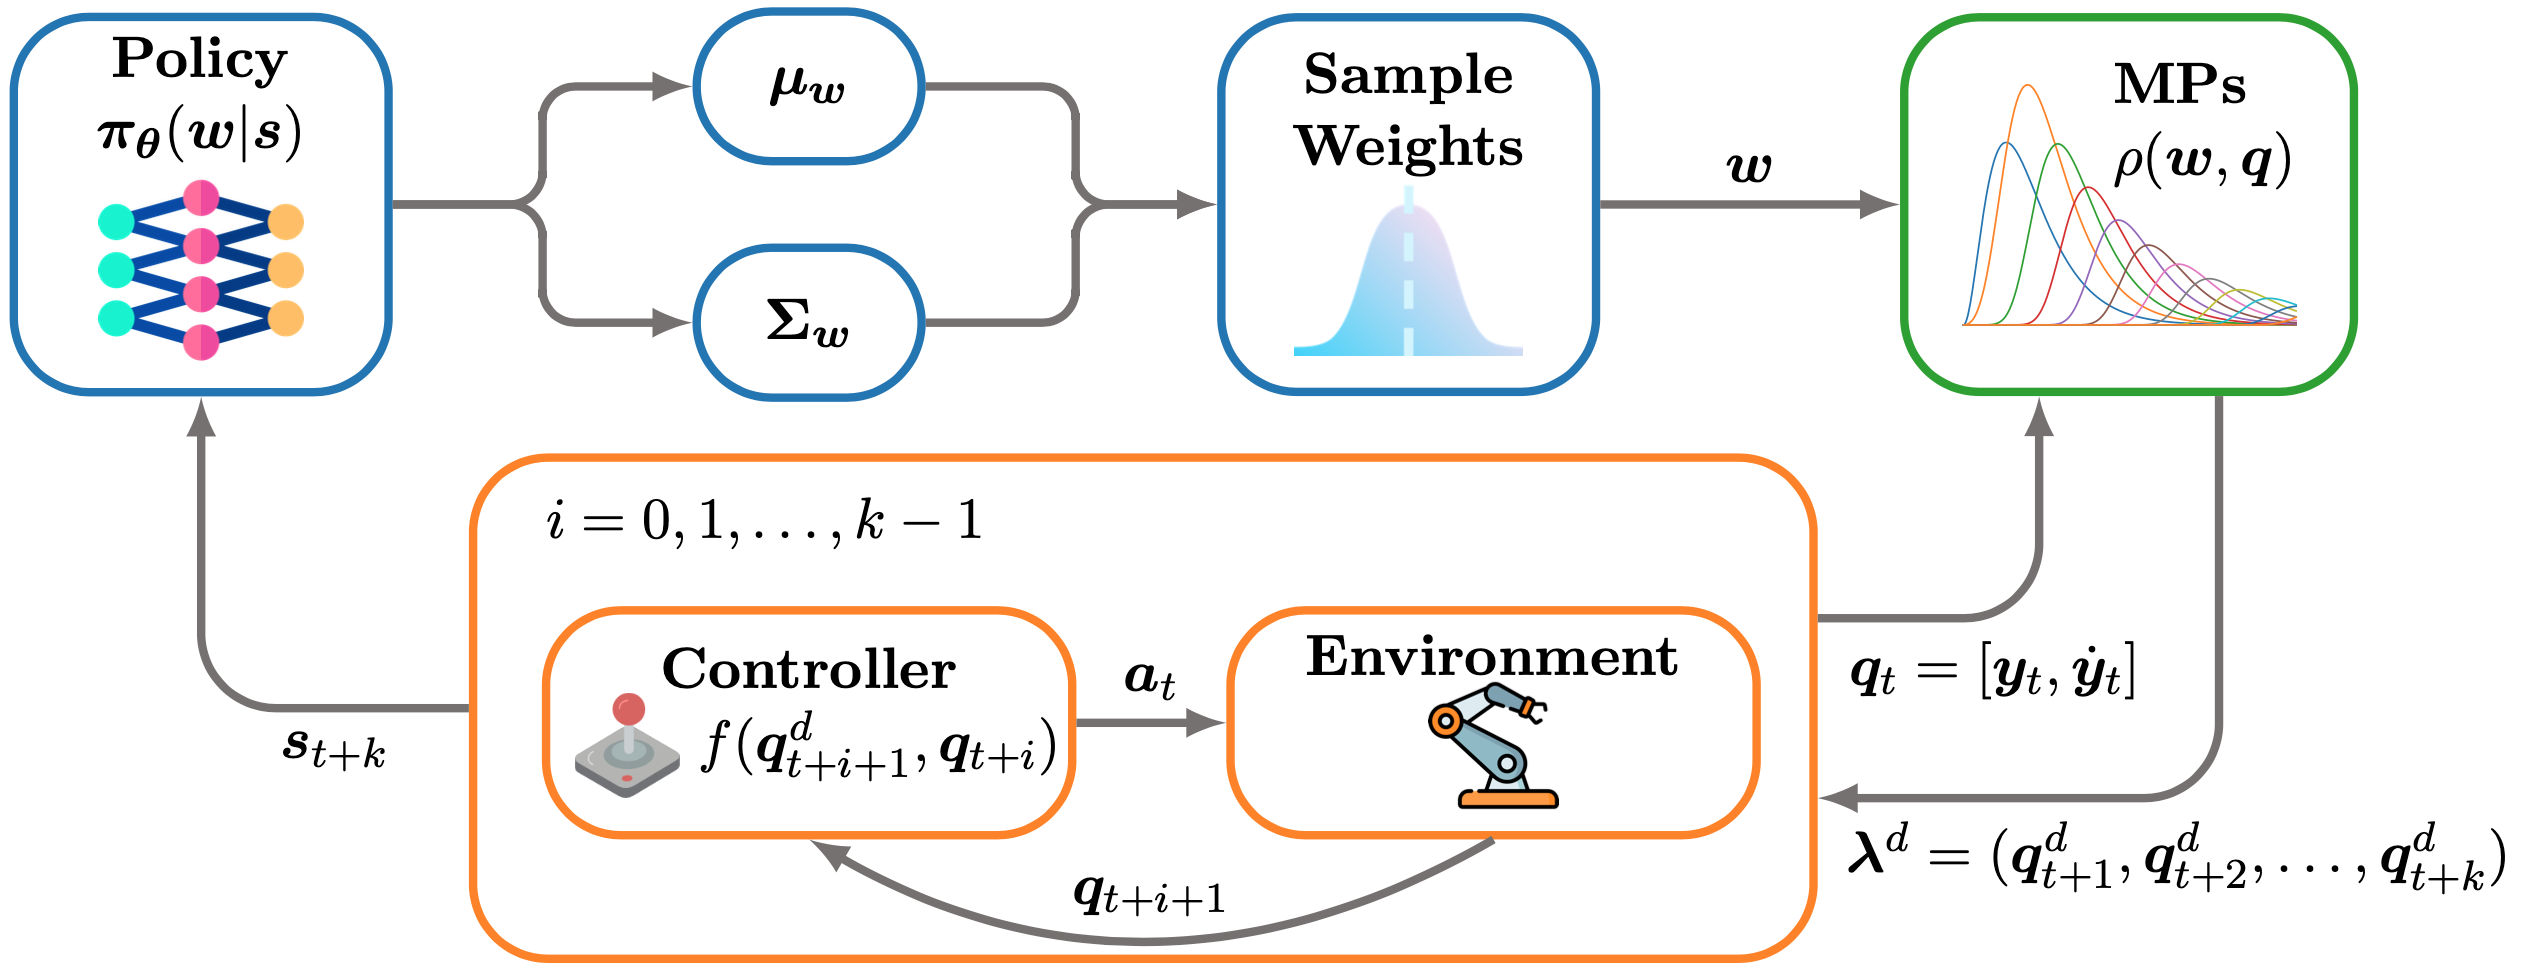
\includegraphics[width=.7\linewidth]{media/mp3.png}
	\begin{itemize}
		\item Contextual MPRL was never used on a real robot\dots will it work?
		\item How big is the sim2real gap?
		\item Do we need replanning?
		\item Is it better than step-based RL (SRL) methods?
	\end{itemize}
\end{frame}



\begin{frame}{Box Pushing}
	\section{Box Pushing}

	\vspace{1cm}
	\begin{columns}
		\begin{column}{0.5\textwidth}
			\begin{itemize}
				\item Goal: Use a stick to push a box to a target pose
				      \begin{itemize}
					      \item Random start pose
					      \item Fixed target pose
				      \end{itemize}
				\item Success:
				      \begin{itemize}
					      \item Position Error < 5cm
					      \item Rotation Error < 0.5 rad

				      \end{itemize}
			\end{itemize}
		\end{column}
		\begin{column}{0.5\textwidth}
			\begin{itemize}
				\item Challenges
				      \begin{itemize}
					      \item Underactuated system
					      \item Complex table-box interactions
					      \item Complex Panda kinematic
					      \item Trajectories must be safe and executable
				      \end{itemize}
			\end{itemize}
		\end{column}


	\end{columns}
	\center
	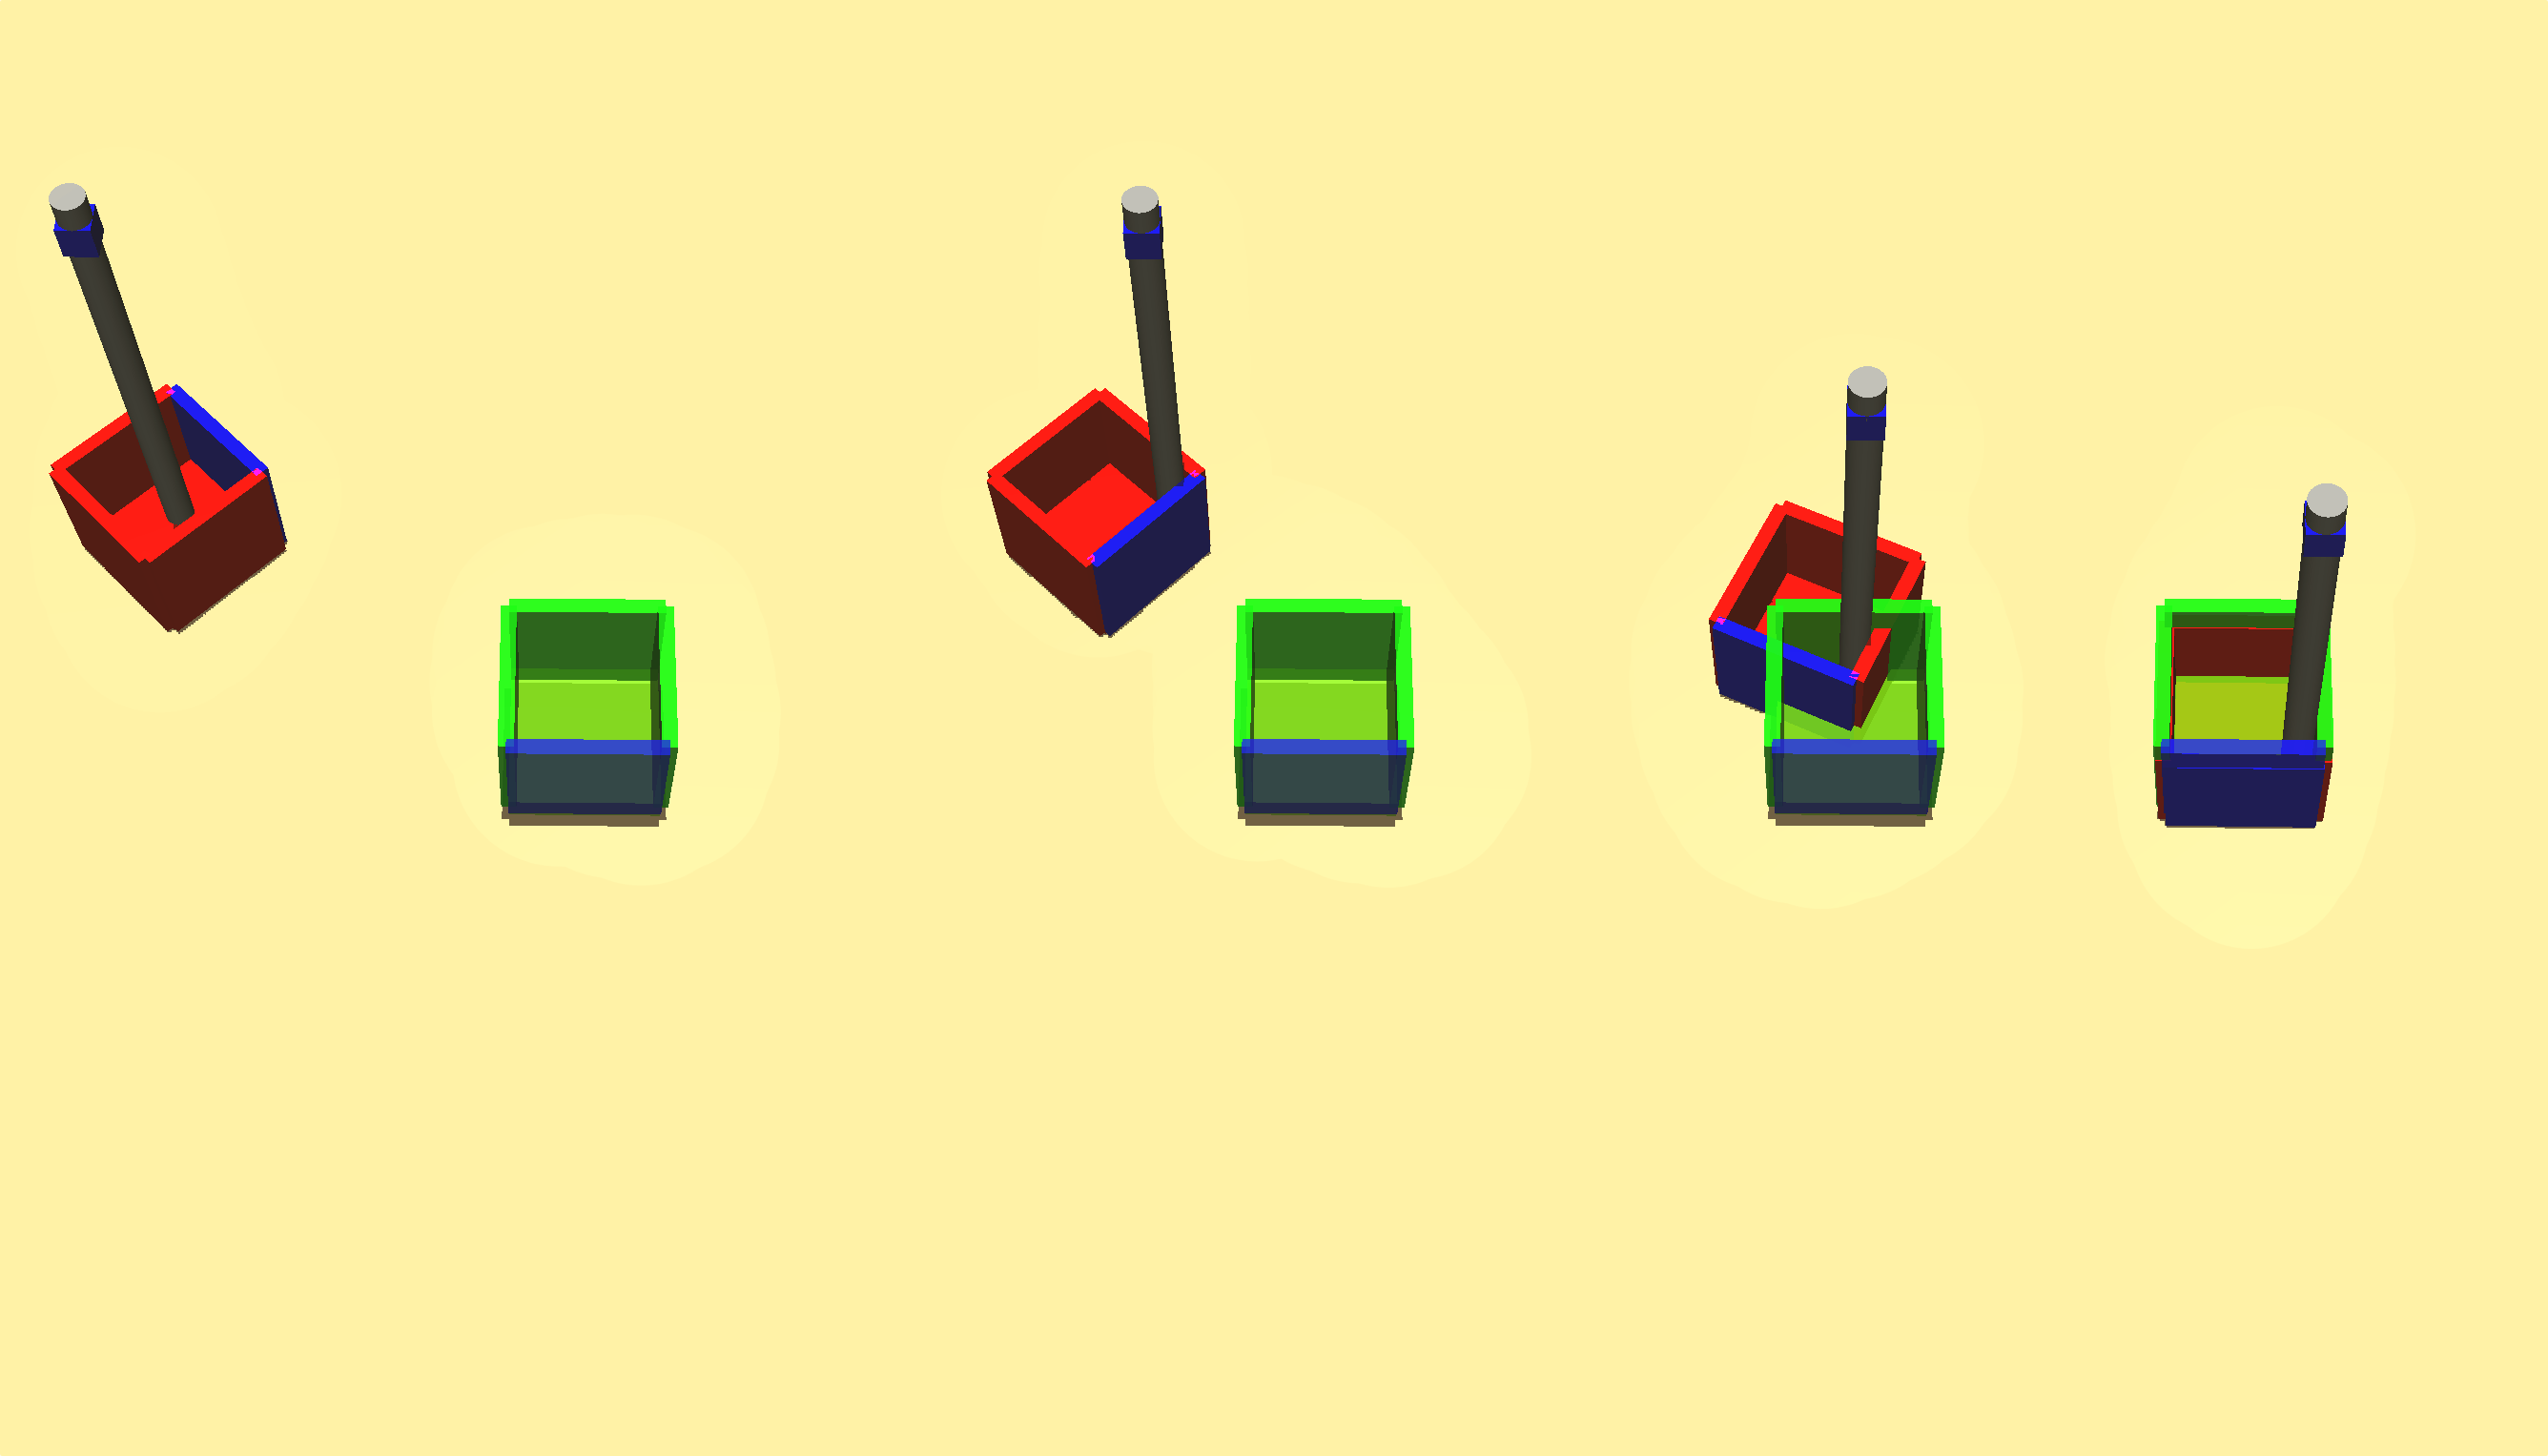
\includegraphics[height=3cm]{media/2dboxpushing.png}
	\vspace{.1cm}\\
	Box Pushing is a challenging benchmark problem for motion primitive reinforcement learning.
\end{frame}


\begin{frame}{How to get RL into the real World}
	\begin{itemize}
		\item Three important Approaches to Real-World RL
		      \begin{itemize}
			      \item Training on the Robot
			      \item Fine-Tuning
			      \item \textbf{Sim2Real}
		      \end{itemize}
		\item Sim2Real is a good fit for MP3 and the simplest to implement
		\item Problem: Sim2Real Gap
		\item Solution: Domain Randomization
		      \begin{itemize}
			      \item Friction $\mu \sim 0.43 \pm 0.1$ \quad (System Dynamics)
			      \item Box Position $x_\text{obs} \sim x \pm 5$cm \quad (Observations)
			      \item Controller P-Gain $k_p \sim k_p^* \pm 68$ \quad (Actions)
		      \end{itemize}

	\end{itemize}

\end{frame}



\section{Experiment 1}
\subsection{Experiment 1}

\begin{frame}{Experiment 1: Setup}

	\begin{center}
		\vspace{1cm}
		\textbf{How well does MP3 work with and without Domain Randomization?}
	\end{center}

	\begin{columns}[t]
		\begin{column}{0.5\textwidth}
			\vspace{.1cm}
			\begin{itemize}
				\item 5 Policies
				      \begin{itemize}
					      \item MP3 Blackbox (with and without DR)
					      \item MP3 Replanning (with and without DR)
					      \item SRL (without DR)
				      \end{itemize}
				\item 16 Starting Poses
				      \begin{itemize}
					      \item 4 Start Positions
					      \item 4 Rotations per Position
				      \end{itemize}
				\item 5 Repetitions per Pose
				\item 400 Episodes in total
			\end{itemize}
		\end{column}
		\begin{column}{0.5\textwidth}
			\vspace{.1cm}
			\includegraphics[width=\textwidth]{../latex/figures/workspace.JPG}
		\end{column}


	\end{columns}
\end{frame}

\subsection{Experiment 1: Blackbox Video}
\begin{frame}{Experiment 1: Blackbox with DR Video}
	\begin{columns}[t]
		\column{0.05\textwidth}
		\column{0.7\textwidth}
		\vspace{1cm}
		\movie[width=\linewidth, height=0.5625\linewidth, poster, showcontrols]{Click to play}{media/122bb-zoom.mov}

	\end{columns}
\end{frame}

\begin{frame}{Experiment 1: Blackbox Trajectories}

	\begin{columns}[t]
		\begin{column}{0.3\textwidth}
			\vspace{1cm}
			\begin{itemize}
				\item Smooth trajectories
				\item Both Trajectories combine small/slow and big/fast movements
				\item DR causes wider, more robust Trajectory
			\end{itemize}
		\end{column}
		\begin{column}{0.7\textwidth}
			\vspace{1cm}
			\includegraphics[width=\textwidth]{../latex/figures/traj_results-2024-08-23_sweep122-bb-128.pdf}\\
			\includegraphics[width=\textwidth]{../latex/figures/traj_results-2024-08-23_sweep121-bb-128_cleaned.pdf}\\
		\end{column}
	\end{columns}
\end{frame}


\subsection{Experiment 1: Results}
\begin{frame}{Experiment 1: Blackbox Results}

	\begin{columns}[t]
		\begin{column}{0.3\textwidth}
			\vspace{1cm}
			\begin{itemize}
				\item 65\% success with DR
				\item 46\% success without DR
				\item 100\% correct position
				\item Noticeable Modes in Rotation Error
				\item Some DR Episodes are very good
			\end{itemize}
		\end{column}
		\begin{column}{0.7\textwidth}
			\vspace{1cm}
			\includegraphics[width=\textwidth]{../latex/figures/results-2024-08-23_sweep122-bb-128.pdf} \\
			\includegraphics[width=\textwidth]{../latex/figures/results-2024-08-23_sweep121-bb-128_cleaned.pdf}\\
		\end{column}
	\end{columns}
\end{frame}

\subsection{Experiment 1: MP3 Replanning Video}
\begin{frame}{Experiment 1: MP3 Replanning DR Video}

	\begin{columns}[t]
		\column{0.05\textwidth}
		\column{0.7\textwidth}
		\vspace{1cm}


		\movie[width=\linewidth, height=0.5625\linewidth, poster, showcontrols]{Click to play}{media/122replan.mov}

	\end{columns}
\end{frame}
\begin{frame}{Experiment 1: MP3 Replanning Trajectories}

	\begin{columns}[t]
		\begin{column}{0.3\textwidth}
			\vspace{1cm}
			\begin{itemize}
				\item Smooth trajectories
				\item Replanning happens every full second
				\item Noticeable Drops in Velocity at 2s, 4s.
				\item DR learns to break contact when switching corners
			\end{itemize}
		\end{column}
		\begin{column}{0.7\textwidth}
			\vspace{1cm}
			\includegraphics[width=\textwidth]{../latex/figures/traj_results-2024-07-29_sweep122-replan-long-1500-128-full.pdf} \\
			\includegraphics[width=\textwidth]{../latex/figures/traj_results-2024-07-29_sweep121-replan-long-1500-128-full.pdf} \\
		\end{column}
	\end{columns}
\end{frame}

\subsection{Experiment 1: Results}
\begin{frame}{Experiment 1: MP3 Replanning Results}
	\begin{columns}[t]
		\begin{column}{0.3\textwidth}
			\vspace{1cm}
			\begin{itemize}
				\item \textbf{94\% success with DR}
				\item 51\% success without DR
				\item 90° Error common without DR
				\item With DR, all but one start Pose successful
			\end{itemize}
		\end{column}
		\begin{column}{0.7\textwidth}
			\vspace{1cm}
			\includegraphics[width=\textwidth]{../latex/figures/results-2024-07-29_sweep122-replan-long-1500-128-full.pdf}
			\includegraphics[width=\textwidth]{../latex/figures/results-2024-07-29_sweep121-replan-long-1500-128-full.pdf}\\
		\end{column}
	\end{columns}
\end{frame}


\subsection{Experiment 1: Step-Based Video}
\begin{frame}{Experiment 1: Step-Based Video}

	\begin{columns}[t]
		\column{0.05\textwidth}
		\column{0.7\textwidth}
		\vspace{1cm}
		\movie[width=\linewidth, height=0.5625\linewidth, poster, showcontrols]{Click to play}{media/trpl_party.mov}

	\end{columns}
\end{frame}

\subsection{Experiment 1: Step-Based Video}
\begin{frame}{Experiment 1: Step-Based Video}


	\vspace{1cm}
	Let's try that again with reduced gains and more time
	\begin{columns}[t]
		\column{0.05\textwidth}
		\vspace{1cm}
		\column{0.7\textwidth}
		\movie[width=\linewidth, height=0.5625\linewidth, poster, showcontrols]{Click to play}{media/trpl.mov}
	\end{columns}

\end{frame}
\begin{frame}{Experiment 1: Step-Based Trajectories}

	\begin{columns}[t]
		\begin{column}{0.3\textwidth}
			\vspace{1cm}
			\begin{itemize}
				\item Noisy commands
				\item Robot is effective in smoothing the trajectory
				\item $\approx0.4$m/s max end-effector velocity
				\item But only $\approx0.2$m/s most of the time
				\item Go to target, rotate, oscillate
			\end{itemize}
		\end{column}
		\begin{column}{0.7\textwidth}
			\vspace{1cm}
			\includegraphics[width=\textwidth]{../latex/figures/traj_results-2024-08-11_sweep123-trpl-slow.pdf}
		\end{column}
	\end{columns}
\end{frame}


\subsection{Experiment 1: Results}
\begin{frame}{Experiment 1: Step-Based Results}

	\begin{columns}[t]
		\begin{column}{0.3\textwidth}
			\vspace{1cm}
			\begin{itemize}
				\item 96\% success without DR
				\item Unimodal Position and Rotation Error
				\item More pronounced Position Error
			\end{itemize}
		\end{column}
		\begin{column}{0.7\textwidth}
			\vspace{1cm}
			\includegraphics[width=\textwidth]{../latex/figures/results-2024-08-11_sweep123-trpl-slow.pdf}
		\end{column}
	\end{columns}
\end{frame}

\subsection{Experiment 1: Discussion}
\begin{frame}{Experiment 1: Discussion}

	\begin{columns}[t]
		\begin{column}{0.3\textwidth}
			\vspace{1em}
			\begin{itemize}
				\item MP3 works
				\item Replanning helps
				\item DR helps
				\item SRL performed very well, but\dots
			\end{itemize}
		\end{column}
		\begin{column}{0.7\textwidth}
			\vspace{1cm}
			\begin{center}

				\begin{tabular}{rccc}
					               & \textbf{Blackbox} & \textbf{Replanning} & \textbf{Step-Based} \\
					\toprule
					\textbf{No DR} & 46\%              & 51\%                & 96\%                \\
					\textbf{DR}    & 65\%              & 94\%                & ---
				\end{tabular}
			\end{center}
		\end{column}
	\end{columns}
\end{frame}

\subsection{Experiment 2: Motivation}
\begin{frame}{Experiment 2 \& 3: Motivation}

	\vspace{1cm}
	\begin{columns}
		\begin{column}{0.5\textwidth}
			\begin{itemize}
				\item Why was SRL so jittery?
				\item Why was SRL sometimes so far off, while still being ``successful''?
				\item Maybe its our Motion Capture\dots
			\end{itemize}
		\end{column}
		\begin{column}{0.5\textwidth}
			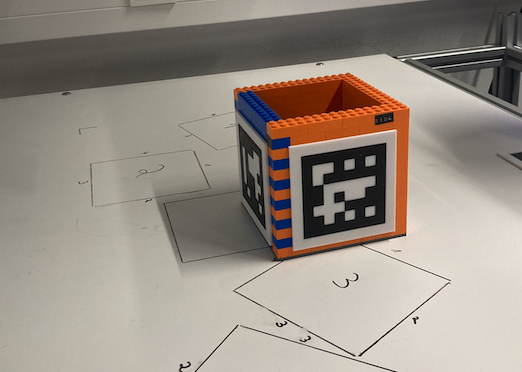
\includegraphics[width=\textwidth]{media/trpl_8cm.png}\\
		\end{column}
	\end{columns}
\end{frame}
\subsection{Experiment 2: Motivation}
\subsection{Experiment 2: Motivation}
\begin{frame}{Experiment 2 \& 3: Motion Capture Error}

	\vspace{1cm}
	\begin{columns}
		\begin{column}{0.3\textwidth}
			\begin{itemize}
				\item We can use the experiment data to analyze Motion Capture Error.
				\item We use the same four starting positions over and over
				\item The camera moves slightly between lab days
				\item Two Kinds of Error:
				      \begin{itemize}
					      \item Offset $\pm 3$cm between Experiments
					      \item Noise $\pm 1$cm within an Experiment
				      \end{itemize}
			\end{itemize}
		\end{column}
		\begin{column}{0.7\textwidth}
			\includegraphics[width=\linewidth]{../latex/figures/mocap_pos_scatter.pdf} \\
		\end{column}
	\end{columns}
\end{frame}
\section{Experiment 2}
\subsection{Experiment 2: Results}
\begin{frame}{Experiment 2}

	\begin{columns}[t]
		\begin{column}{0.3\textwidth}
			\vspace{.1cm}
			\begin{itemize}
				\item Increase position noise by adding $\pm 5$cm of uniform noise to the observed box position
				\item Replanning with DR actually improves to 100\% success
				\item SRL drops to 81\% success
				\item SRL becomes very noisy
			\end{itemize}
		\end{column}
		\begin{column}{0.6\textwidth}
			\vspace{1cm}
			\includegraphics[width=.8\textwidth]{../latex/figures/traj_results-2024-08-15_sweep123-trpl-5cm.pdf}\\
			\vspace{-1cm}
			\includegraphics[width=\textwidth]{../latex/figures/results-2024-08-15_sweep122-replan-5cm.pdf}\\
			\includegraphics[width=\textwidth]{../latex/figures/results-2024-08-15_sweep123-trpl-5cm.pdf}\\
		\end{column}
	\end{columns}
\end{frame}

\section{Experiment 3}
\subsection{Experiment 3: Results}
\begin{frame}{Experiment 3}

	\begin{columns}[t]
		\begin{column}{0.3\textwidth}
			\vspace{1cm}
			\begin{itemize}
				\item Add constant offset of $10$cm to observed box position
				\item Replanning with DR at 100\% success again
				\item SRL drops to 0\% success
			\end{itemize}
		\end{column}
		\begin{column}{0.6\textwidth}
			\vspace{1cm}
			\includegraphics[width=\textwidth]{../latex/figures/results-2024-08-19_sweep123-replan-offset.pdf}\\
			\includegraphics[width=\textwidth]{../latex/figures/results-2024-08-19_sweep123-trpl-offset.pdf}\\
		\end{column}
	\end{columns}
\end{frame}



\section{Discussion}
\begin{frame}{Discussion}

	\begin{itemize}
		\item We probably overestimated SRL's position accuracy
		\item Mocap Noise could explain the unstable SRL trajectories
		\item MP3 Replanning handles Mocap Offsets and Noise remarkably well
	\end{itemize}
\end{frame}


\appendix
\beginbackup{}
\begin{frame}{SRL Accelerations in Simulation}

	\vspace{1cm}
	\centering
	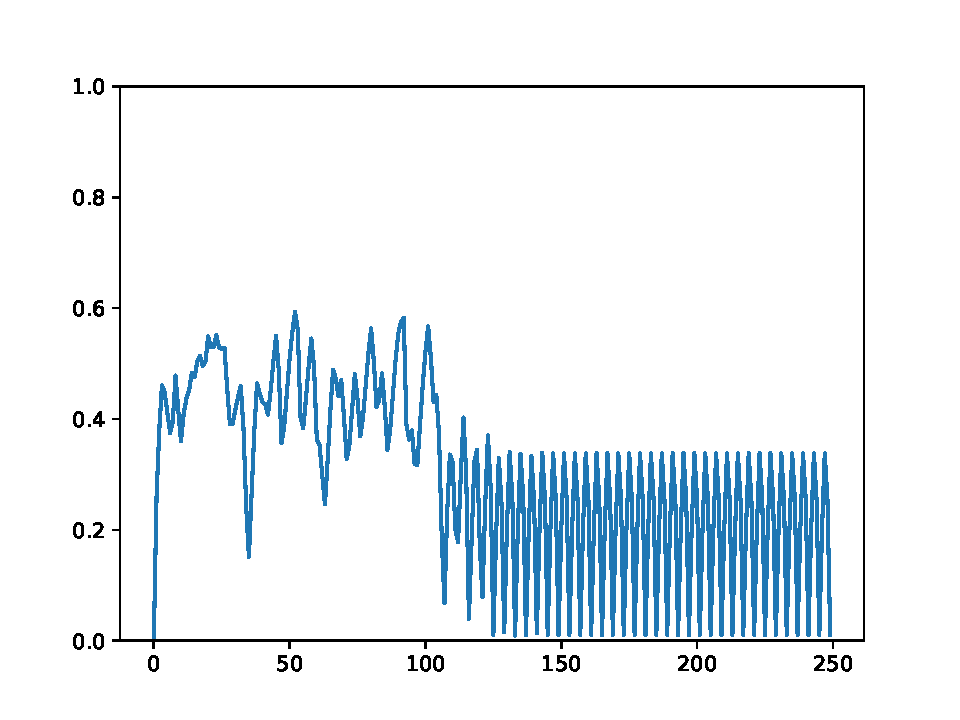
\includegraphics[width=.6\textwidth]{media/trpl_sim.pdf} \\
\end{frame}

\subsection{Experiment 1: How MP3 fails}
\begin{frame}{Experiment 1: How MP3 fails}

	\begin{columns}[t]
		\begin{column}{0.5\textwidth}
			\vspace{1cm}
			\begin{itemize}
				\item Distinct Modes in Rotation Error
				      \begin{itemize}
					      \item Failure to transition from corner to Corner (90°)
					      \item Trying to push the sides of the box (45°)
				      \end{itemize}
				\item We saw that DR policies learned to mitigate this.
				      \begin{itemize}
					      \item Wide Movements
					      \item Avoid Pushing the flat Sides
					      \item Break Contact when transitioning between corners
				      \end{itemize}
			\end{itemize}
		\end{column}
		\begin{column}{0.5\textwidth}
			\vspace{1cm}
			\includegraphics[width=\textwidth]{../latex/figures/results-2024-08-23_sweep122-bb-128.pdf} \\
			\includegraphics[width=\textwidth]{../latex/figures/results-2024-08-23_sweep121-bb-128_cleaned.pdf}\\
			\includegraphics[width=\textwidth]{../latex/figures/results-2024-07-29_sweep121-replan-long-1500-128-full.pdf}\\
		\end{column}
	\end{columns}
\end{frame}

\begin{frame}{Experiment 1: How MP3 Replanning with DR fails}
	\subsection{Experiment 1: How MP3 Replanning fails}
	\begin{center}
		\includegraphics[width=.3\linewidth]{../latex/figures/failure_0.pdf}
		\includegraphics[width=.3\linewidth]{../latex/figures/failure_50.pdf}
		\vspace{-.5cm}
		\includegraphics[width=.3\linewidth]{../latex/figures/failure_100.pdf} \\
		\includegraphics[width=.3\linewidth]{../latex/figures/failure_150.pdf}
		\includegraphics[width=.3\linewidth]{../latex/figures/failure_200.pdf}
		\includegraphics[width=.3\linewidth]{../latex/figures/failure_250.pdf} \\
		Everything looks good\dots until the last replan step.

		Maybe give it more weight during training?
	\end{center}
\end{frame}
\begin{frame}{Box Pushing --- Clipping }
	\begin{columns}
		\begin{column}{0.4\textwidth}
			\vspace{.1cm}
			\[ \text{Reward}_{\text{clipping}} := \sum_t \left\Vert x_t - x_t^\text{clipped} \right\Vert \]
			\begin{itemize}
				\item Idea: Penalize the agent for \textbf{leaving the working area}
				\item Outside of the working area, the policy is \textbf{ineffective}
				\item Without the reward, the agent\dots
				      \begin{itemize}
					      \item spent 80\% of its time outside the working area
					      \item never learned to correct this
					      \item exceeded the maximum speed $v_\text{max}$
				      \end{itemize}
			\end{itemize}
		\end{column}
		\begin{column}{0.6\textwidth}
			\vspace{.1cm}
			\center
			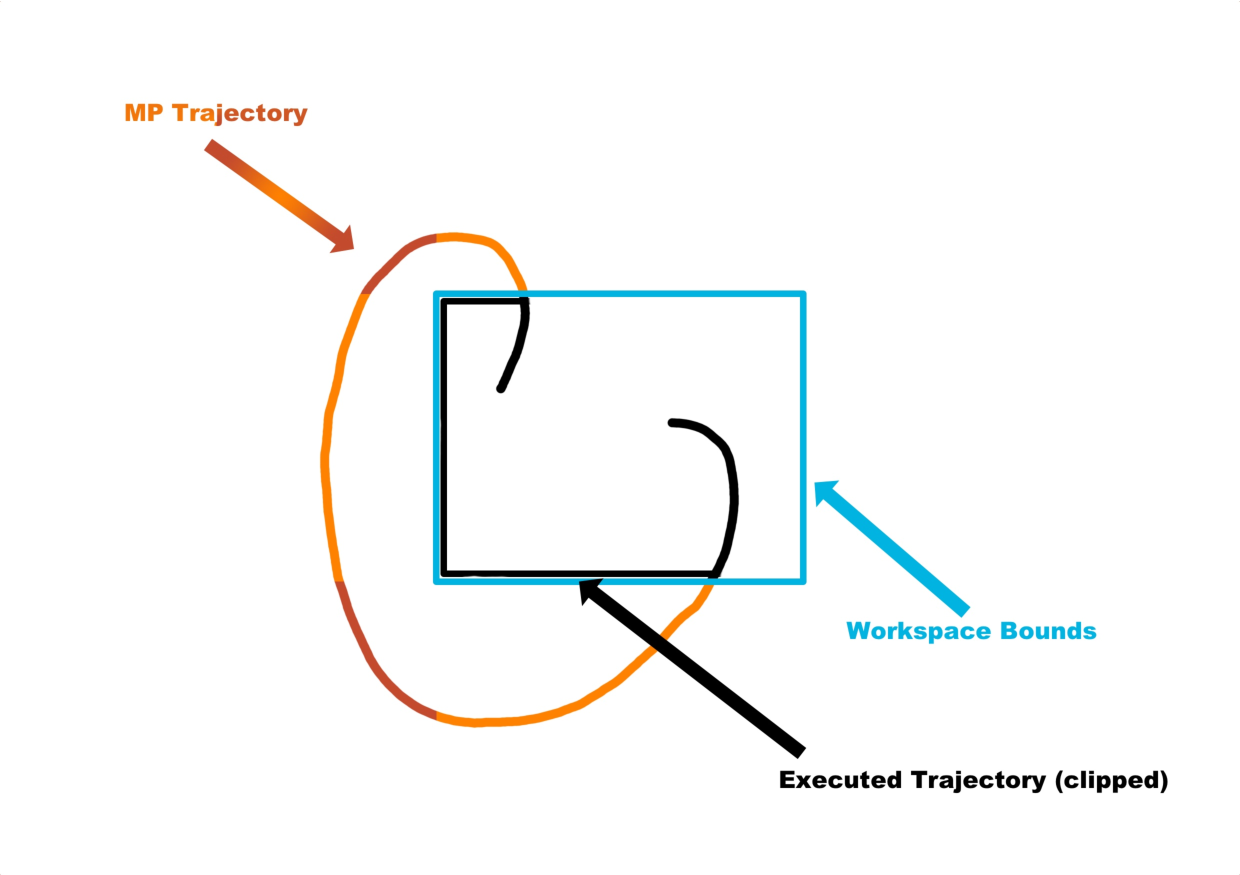
\includegraphics[width=\linewidth]{media/workspace_clipping.pdf}

		\end{column}
	\end{columns}
\end{frame}

\begin{frame}{Box Pushing --- Clipping}

	\begin{columns}
		\begin{column}{0.4\textwidth}
			\vspace{1cm}
			\begin{itemize}
				\item Clipping penality has a big effect on performance
				\item Every MP Env should have one
			\end{itemize}
		\end{column}
		\begin{column}{0.6\textwidth}
			\vspace{.2cm} \\
			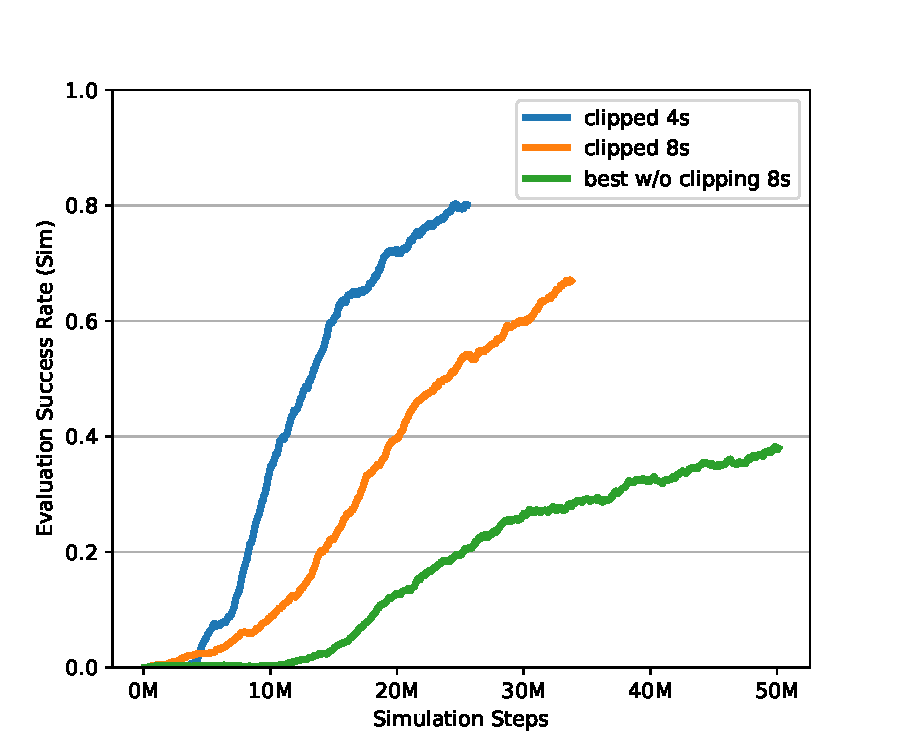
\includegraphics[width=\linewidth]{media/clipping_reward.pdf}

		\end{column}
	\end{columns}
\end{frame}

\begin{frame}{Box Pushing}

	\begin{columns}[t]
		\begin{column}{0.4\textwidth}
			\vspace{1cm}
			\begin{itemize}
				\item Goal: Use a finger to push a box to a target pose
				      \begin{itemize}
					      \item Random start pose
					      \item Fixed target pose
				      \end{itemize}
				\item Action space: 2D finger positions
				\item Observation:
				      \begin{itemize}
					      \item Finger position
					      \item Box quaternion + noisy position
				      \end{itemize}
				\item Success
				      \begin{itemize}
					      \item $\text{err}_{position} \leq 5 \text{cm}$
					      \item $\text{err}_{rotation} \leq 0.5 \text{rad}$
					      \item $\max_t(v_t) < v_\text{max}$
				      \end{itemize}
			\end{itemize}
			\vspace{1em}
		\end{column}
		\begin{column}{0.5\textwidth}
			\vspace{.5cm}
			\[
				\begin{aligned}
					\text{Reward} & := \textcolor{kit-blue100}{\text{Final Euclidean Distance}}                         \\
					              & +  \textcolor{kit-blue100}{\text{Final Rotational Distance}}                        \\
					              & +  \textcolor{kit-blue100}{\mathds{1} \left\{\text{success}\right\} }               \\
					              & -  \textcolor{kit-green100}{\max_t\  \text{step}(v_t)}                              \\
					              & -  \textcolor{kit-lila100}{\sum_t \left\Vert x_t - x_t^\text{clipped} \right\Vert } \\
					\\
					step(v) :=    & 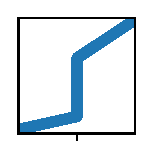
\includegraphics[scale=.4]{media/step.pdf}                                          \\
				\end{aligned}
			\]

		\end{column}
	\end{columns}
	\center
	Our reward includes \textcolor{kit-blue100}{sparse}, \textcolor{kit-green100}{non-markovian} and \textcolor{kit-lila100}{dense} components.
\end{frame}

\subsection{Making it work in Simulation}
\begin{frame}{Box Pushing --- In Simulation}

	\begin{columns}[t]
		\begin{column}{0.4\textwidth}
			\vspace{1cm}
			\begin{itemize}
				\item Box Pushing is \textbf{hard}.
				      \begin{itemize}
					      \item It took long to get $60-80$\% success in sim
					      \item 127 Sweeps so far, 2628 policies trained
					      \item $\approx 25-50\text{M}$ sim steps per policy
					      \item $\approx 60-120\text{K}$ 4s trajectories
				      \end{itemize}
				\item So many parameters:
				      \begin{itemize}
					      \item Reward coefficients
					      \item Maximum Speed $v_{\max}$
					      \item Amount of randomization
					      \item Episode Length
					      \item MP Parameters
					      \item TRPL Hyperparameters
				      \end{itemize}
			\end{itemize}
		\end{column}
		\begin{column}{0.5\textwidth}
			\vspace{.2cm} \\
			\center
			\includegraphics[width=.5\linewidth]{../fancy_gym/sweeps.pdf} \\

		\end{column}
	\end{columns}
\end{frame}

\subsection{Making it work on the real Robot}

\begin{frame}{Box Pushing --- Making it work on the real Robot}
	\begin{columns}
		\begin{column}{0.5\textwidth}
			\begin{itemize}
				\item No controller tracks perfectly
				\item The agent will \textbf{adapt} to the simulated controller under- or overshooting.
				\item Also the real robot trajectory has artifacts because of the 7DoF kinematics
				\item \textbf{Tuning for the real robot is crucial!}
			\end{itemize}
		\end{column}
		\begin{column}{0.5\textwidth}
			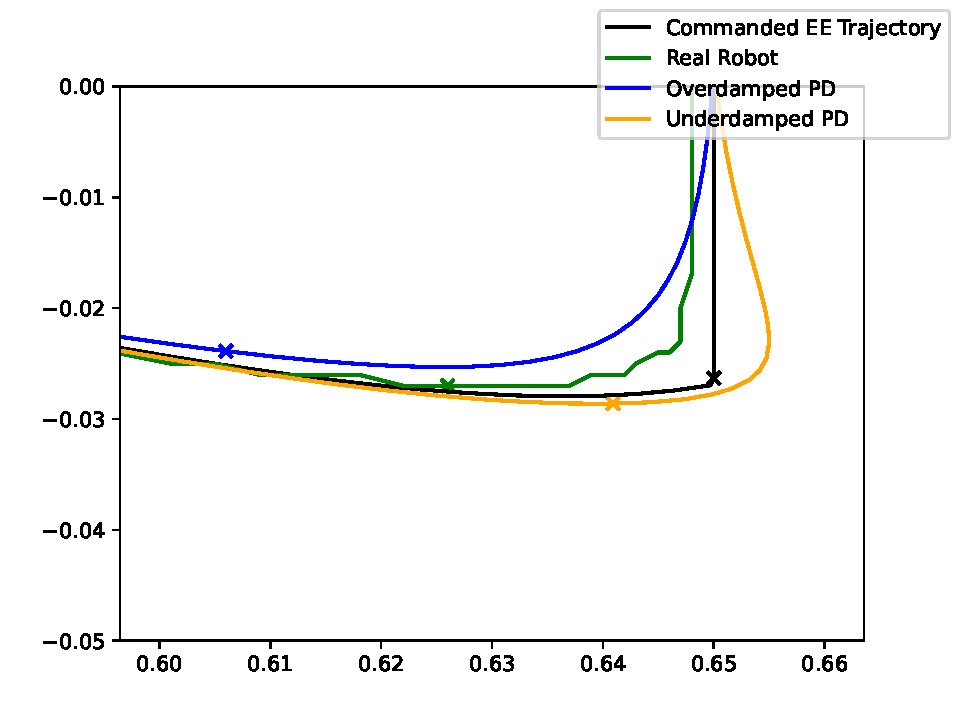
\includegraphics[width=\linewidth]{media/traj_error.pdf}
		\end{column}
	\end{columns}

\end{frame}
\begin{frame}{Box Pushing --- Making it work on the real Robot}
	\begin{columns}
		\begin{column}{0.5\textwidth}
			\begin{itemize}
				\item Our approach:
				      \begin{itemize}
					      \item Record real-robot executions
					      \item Optimize simulation PD parameters using bayesian optimization
					      \item Choose a lower/higher P-gain
					      \item Sample $Kp \sim \text{U}(Kp^-, Kp^+)$ during training
				      \end{itemize}

				      \[
					      \min_{kp, kd, mass} \sum_t \left\Vert x_t^\text{real} - x_t^\text{sim}(kp, kd, mass) \right\Vert
				      \]
			\end{itemize}
		\end{column}

		\begin{column}{0.5\textwidth}
			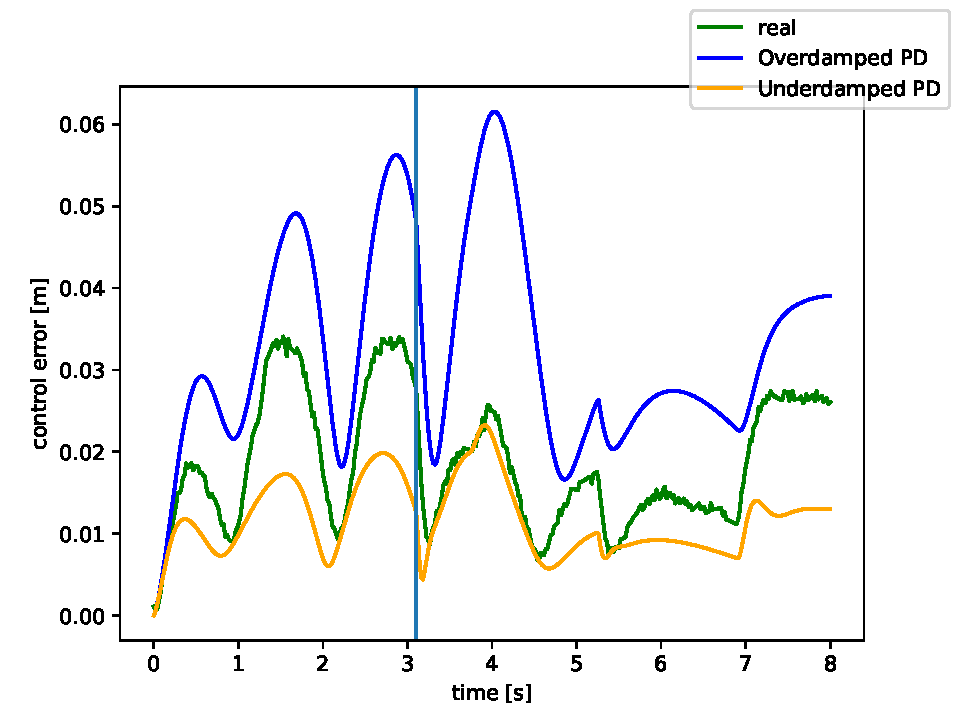
\includegraphics[width=\linewidth]{media/ctrl_error.pdf}\\
		\end{column}
	\end{columns}

\end{frame}

\section{Rollout Architecture}
\begin{frame}{Rollout Architecture}
	\begin{columns}
		\begin{column}{0.45\textwidth}
			\vspace{1cm}
			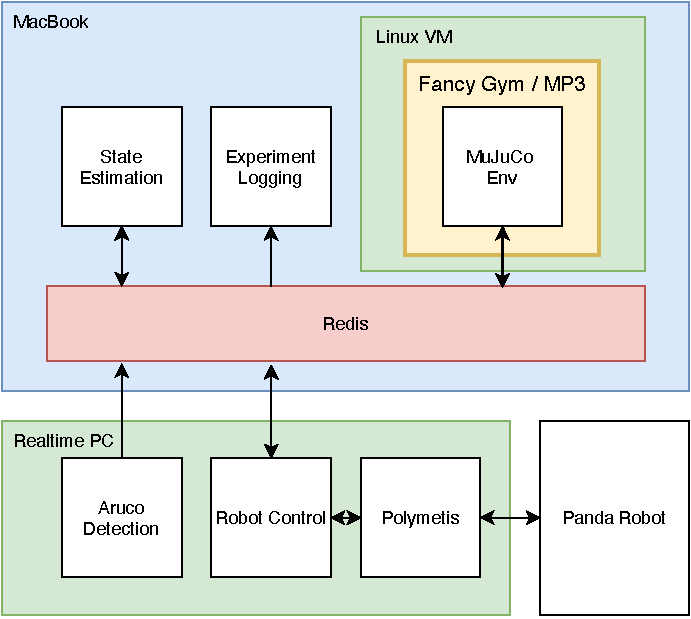
\includegraphics[width=\linewidth]{media/Architecture2.pdf}

		\end{column}
		\begin{column}{0.35\textwidth}
			\vspace{1cm}
			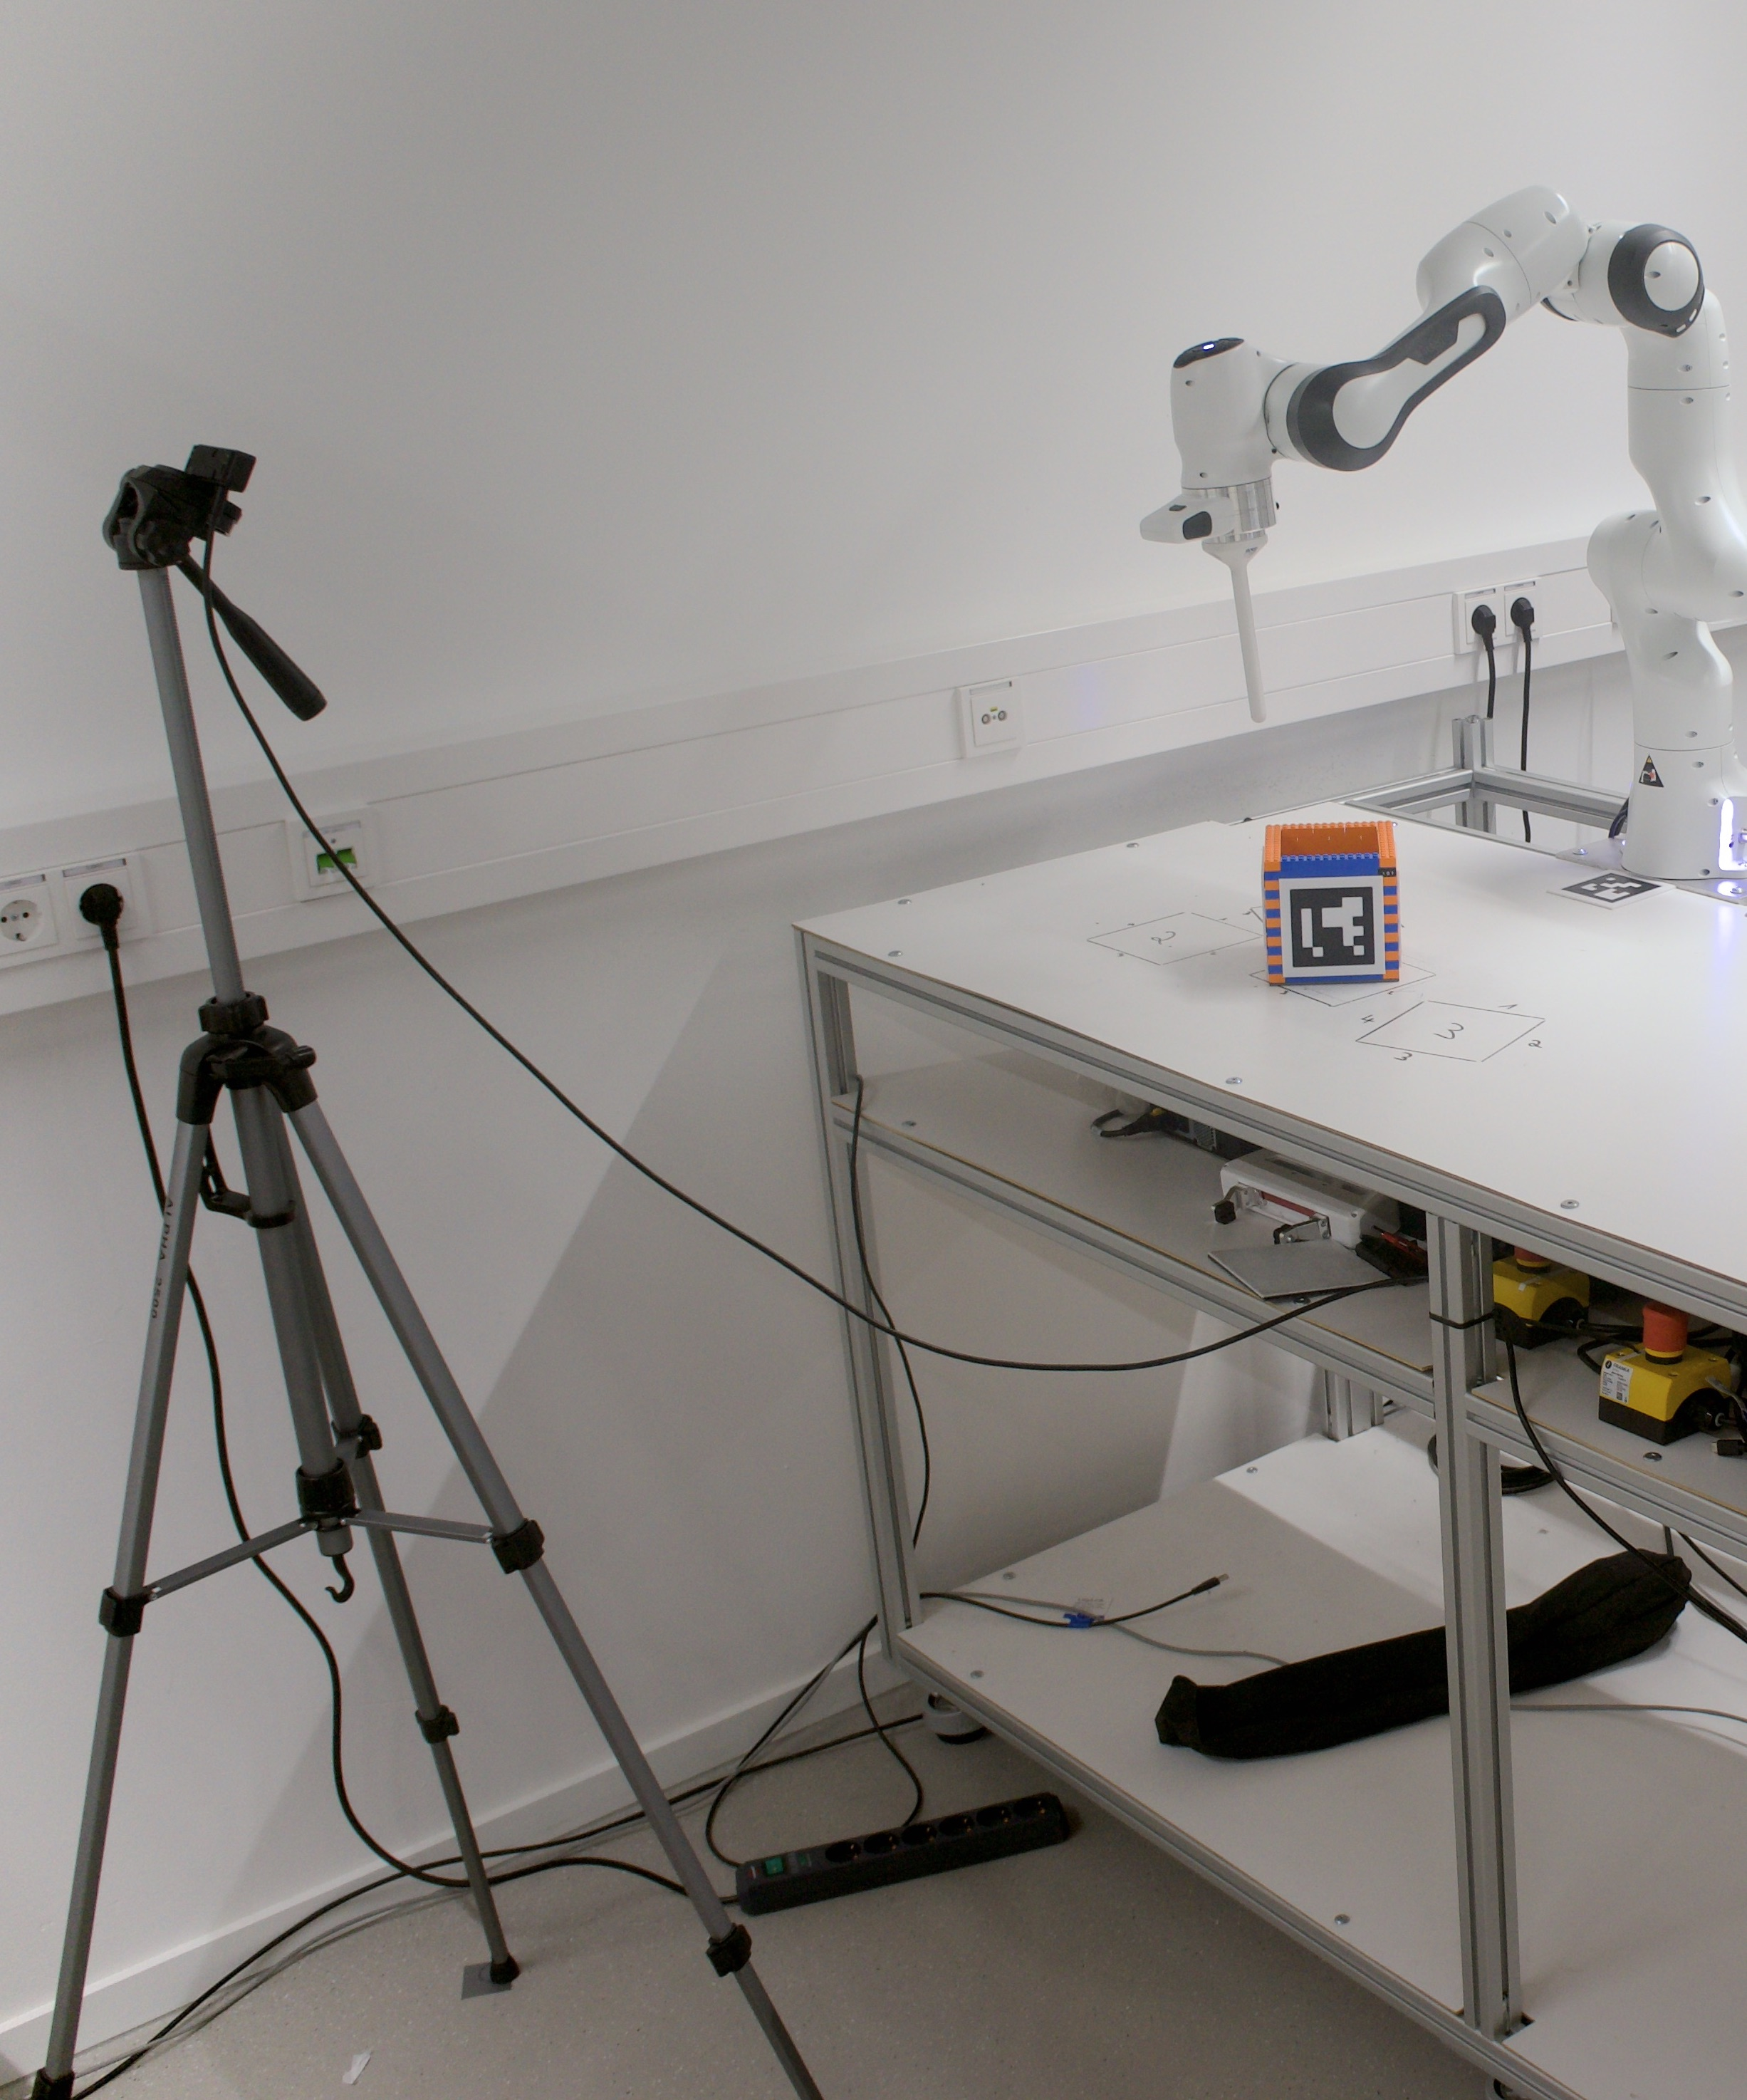
\includegraphics[width=\linewidth]{media/labsetup2.jpg}

		\end{column}
	\end{columns}

\end{frame}


\backupend{}

\end{document}
